\documentclass[12pt]{article}
\usepackage{geometry}
\usepackage{xcolor}
\usepackage{hyperref}
\usepackage[utf8]{inputenc}
\usepackage{tabto}
\usepackage{graphicx}
\usepackage{biblatex}
\usepackage{comment}
\addbibresource{bibliography.bib}
\graphicspath{ {./images/} }
\hypersetup{
colorlinks=false,
linktoc=all
}
\geometry{
a4paper,
left=30mm,
top=30mm,
right=30mm,
bottom=40mm
}
\newcommand{\sentence}{} % New sentence
\newcommand{\final}{} % Mark a section as finished
\title{Animation Vectorization and Compression}
\author{Bassam Helal}
\date{September 2020}
\begin{document}
    % TODO 12-Sep-20 Remove black background and white text
    \pagecolor{black}
    \color{white}

    \pagenumbering{gobble}

    \maketitle

    \begin{center}
        \vspace{8cm}
        
\includegraphics[scale=0.65]{SwanseaUniversityLogo.png}
    \end{center}

    \pagebreak

    \begin{center}
        \section*{Abstract}
    \end{center}

    % TODO 12-Sep-20 Abstract

    \pagebreak

    \renewcommand*\contentsname{
    \begin{center}
        Table of Contents
    \end{center}}

    \tableofcontents

    \pagebreak

    \pagenumbering{arabic}


    \section{Introduction}\label{sec:introduction}

    % A paragraph or so for each of:

    % Project Description
    % Motivation
    % Existing Literature
    % Limitations of the literature that we will attempt to tackle
    % Aims and Objectives
    % Discoveries and results we found after our attempts
    % Section Signposting

    \pagebreak


    \section{Background}\label{sec:background}

    \tab
    This document makes no assumption of the reader's knowledge in computer graphics and its related fields,
    thus, this section will introduce the reader to some of the required knowledge needed for understanding this
    project.
    \sentence
    Firstly, we will introduce raster graphics, ie, the current common standard for graphics data representation.
    We will then introduce its counterpart vector graphics, a different way to store graphics data that is growing in
    popularity and has its own advantages and disadvantages.
    \sentence
    We will then give a brief primer on image compression and some common methods of reducing the overall size
    of an image.
    \sentence
    Finally, we will explain how this all ties into video graphics and describe some of the few differences between
    image graphics and video graphics.

    \subsection{Raster Graphics}\label{subsec:raster-graphics}

    % 1 - 2 sentences for each of:
    % Brief summary of what we will go over (signposting)
    % Pixels, Bitmaps, Image Data Buffers: basically the bare must knows about Raster Graphics
    % Advantages and popularity of Raster Graphics
    % Disadvantages like upscaling, pixelation, size issues with high resolution
    % Brief summary of everything we just mentioned

    \tab
    Raster graphics is the current most popular way of representing and storing graphics data.
    \sentence
    This representation format stores the image data as a grid of pixels, a pixel (picture element) being the color
    of the image at a particular point in the grid.
    \sentence
    Colors can be represented in a variety of ways but the most common is RGB with RGBA also being found in some
    formats.
    \sentence
    Each channel has a bit depth which details the number of possible colors that the channel can contain with 8 bits
    per channel being the current most common but higher values exist as well such as 10 and 12 bits per channel.
    \sentence
    Thus the image data is a 2 dimensional array of pixels which could be 3 or 4 channels of 8 bit values, thus an
    image can also be represented as a 3 dimensional array with the last dimension being 3 or 4 values in size
    representing the 3 or 4 channels of that pixel.
    \sentence
    The resolution of an image is the number of pixels it contains, which is the image's width multiplied by its
    height, higher resolution images have more detail but are also more expensive to store as there is more data.
    \sentence
    Raster graphics are the most popular form of image and generally graphics representation, they allow for easy
    representation and computationally cheap as well since all the data is stored with no extra work needed.
    \sentence
    The main disadvantages of raster graphics have to with image resolution and detail, namely that images will show
    pixelation artifacts when they are displayed at a higher resolution than they are actually stored at, thus the
    image appears to show the raw pixels.
    \sentence
    % TODO 16-Sep-20 Show pixelation images
    To compensate for this, higher and higher resolution images are needed but those come at the cost of size.
    \sentence
    % TODO 16-Sep-20 Explain more about raw size (no compression, so use raw format or just plain numbers)
    \sentence
    % TODO 16-Sep-20 Summarize

    \subsection{Vector Graphics}\label{subsec:vector-graphics}

    % 1 - 2 sentences for each of:
    % Brief summary of what we will go over (signposting)
    % Declarative vs Imperative ie WYSIWYG vs WYSIWYM, describing the image using primitive geometry
    % Advantages of Vector especially in contrast to Raster (size and scalability), mention uses and popularity
    % Disadvantages like portability and light technical stuff like gradients and photographs
    % Brief summary of everything we just mentioned

    % TODO 16-Sep-20 We can make a small table comparing Raster & Vector Graphics for the attributes like size,scalability etc

    \subsection{Image Compression}\label{subsec:image-compression}

    % 1 - 2 sentences for each of:
    % Brief summary of what we will go over (signposting)
    % Fundamentals of Compression (type-agnostic) things like compression rate and lossy-ness or accuracy
    % Lossless Image Compression (PNG, BMP etc)
    % Lossy Image Compression (JPEG, GIF etc)
    % Brief summary of everything we just mentioned

    % TODO 16-Sep-20 We can have an image comparing popular image file types with regards to compression

    \subsection{Video Graphics}\label{subsec:video-graphics}

    % 1 - 2 sentences for each of:
    % Brief summary of what we will go over (signposting)
    % How video is stored and how it relates to Images (mostly the same)
    % Common file types and how they compress and store video data (MP4, MKV, H265 etc)
    % Evidence and proof of why video is expensive (and also popular)
    % Brief summary of everything we just mentioned

    \subsection{Toolchain}\label{subsec:toolchain}

    % 1 - 2 sentences for each of:
    % Brief summary of what we will go over (signposting)
    % Node.js
    % JavaScript, TypeScript (benefits over JS)
    % Supplementaries like Electron, GPU.js, OpenCV etc
    % Brief summary of everything we just mentioned

    % TODO 19-Sep-20 Shorten!
    \tab
    This project uses a variety of popular tools and libraries to achieve its aims and objectives both efficiently
    and quickly, this section will briefly go over the most important tools used.
    \sentence
    This project uses Node.js as its runtime platform, Node.js is a cross-platform runtime environment that executes
    JavaScript code on a machine instead of the usual JavaScript runtime, the browser.
    \sentence
    The choice for Node.js was made paradoxically because of both a familiarity with the runtime and the JavaScript
    ecosystem as well as a strong desire to further enhance our knowledge and experience in both the platform and
    ecosystem.
    \sentence
    Node.js allows us to access the ever-growing JavaScript ecosystem which includes very powerful libraries and
    frameworks for both front-end designs and back-end computationally heavy workloads.
    \sentence
    Node.js uses JavaScript as its runtime language, while JavaScript is a powerful and excellent language for
    rapid-prototyping, it is also a very error-prone language as it has no typing checks in place.
    \sentence
    TypeScript is a programming language that is a strict superset of JavaScript that adds typing features onto
    JavaScript and transpiles to performant, cross-platform compatible JavaScript by means of a TypeScript compiler.
    \sentence
    TypeScript was chosen as the programming language of choice for the project for its many benefits not limited to
    its added type safety.
    \sentence
    The JavaScript ecosystem provides us with some powerful libraries and frameworks for application development,
    this project makes use of some excellent noteworthy tools such as Electron, GPU.js and OpenCV among other tools.
    \sentence
    Electron allows developers to write desktop applications using web technologies, it essentially is a Chromium
    browser with two processes, a front-end process(es) called the "renderer" which is similar to a Chromium web page
    that displays HTML, and a back-end process called the main process which is a Node.js process.
    \sentence
    Electron combines Node.js and Chromium to allow a developer to write a native desktop application using the same
    technologies used on the web, this has its own advantages and disadvantages but in our case, it means we can
    quickly develop a GUI desktop application that can access our Node.js code without resorting to web servers and
    other more complicated means.
    \sentence
    GPU.js is a JavaScript library that allows developers to run code on the host machine's GPU making use of the
    GPGPU (General-Purpose computing on Graphics Processing Units) paradigmGeneral-purpose computing on graphics
    processing units.
    \sentence
    This can allow for very large performance improvements and speedups for computationally expensive mathematical
    computations.
    \sentence
    % TODO 19-Sep-20 OpenCV? We didn't use it too much and this is already getting too long
    \sentence
    In summary, the project uses the Node.js runtime for its large ecosystem, the TypeScript programming language for
    its added type safety benefits, Electron to easily display a GUI and GPU.js to run code on the GPU for additional
    performance when needed.
    \pagebreak


    \section{Related Work}\label{sec:related-work}

    % Here we throw a lot of the current stuff from both research and industry and show their flaws and limitations
    % (which we may or may not have tackled)

    \subsection{Current Research}\label{subsec:current-research}

    % Brief summary of what we will go over (signposting)
    % New Machine Learning methods for Vectorization
    % New Machine Learning methods for Compression
    % Novel approaches and ideas within Vectorization such as mesh gradients etc (no ML)
    % Brief summary of everything we just mentioned

    \subsection{Current Applications}\label{subsec:current-applications}

    % Brief summary of what we will go over (signposting)
    % Adobe Illustrator, Logos, Topography, Medical stuff like X rays etc Potrace
    % Animations and Games using Vector as the development method
    % Current Image \& Video compression algorithms such as PNG, H265 and H266 (no ML)
    % Brief summary of everything we just mentioned

    \subsection{Limitations}\label{subsec:limitations}

    % Brief summary of what we will go over (signposting)
    % Why ML is absolute hot trash
    % Show off the flaws with existing technologies while showing how we tackled (and hopefully beat) them
    % Discuss inherent limitations of this process, such as issues with Vector Graphics and input data being varying etc
    % Brief summary of everything we just mentioned

    \pagebreak


    \section{Implementation}\label{sec:implementation}

    % TODO 15-Sep-20 This may get long and technical, we should try to keep things fairly high level as much as
    %  possible we will also show both Math, pseudocode and pipeline of the overall process and avoid boring low level
    %  details

    \subsection{Pipeline}\label{subsec:pipeline}

    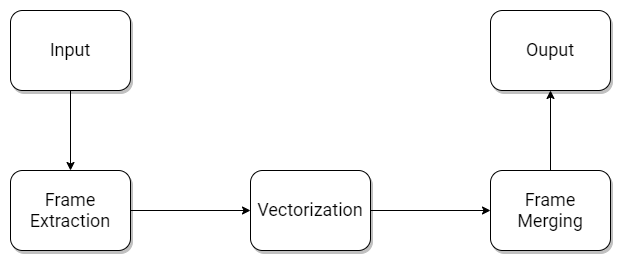
\includegraphics[width=\textwidth]{Pipeline.png}
    % TODO 15-Sep-20 Fix positioning and add a caption, read more here https://cs.overleaf.com/learn/latex/Inserting_Images

    % This pipeline image describes the the project's implementation from a high level view.
    % Each phase of the pipeline is further detailed.

    \subsubsection{Input}

    % An animated cartoon video, particularly one with vectorizable qualities, which we will further detail

    % Low or no use of gradients so it has discrete colors
    % Low or no noise
    % No 3D stuff like shadows and reflections

    % Show examples of good cartoons and have images, so Fairly OddParents, Teen Titans Go as well as some less optimal
    % cartoons like old Tom and Jerry, Hannah Barbera and Ed, Edd n Eddy

    \subsubsection{Frame Extraction}

    \subsubsection{Vectorization}

    % Conversion of each Frame to an SVG which will have a single SVG Path element for each color

    \subsubsection{Frame Merging}

    % SVG Frame Joining which will have some smart compression built-in

    \subsubsection{Output}

    % An SVG Video that is of course highly scalable and has a lower size than the original if upscaled and with
    % very minimal data loss

    \subsection{Vectorization Methods}\label{subsec:vectorization-methods}

    % Here we will explain our story of the last few months, the many approaches and their failures. This section
    % should implicitly show the reader that the problem is very hard, harder than initially thought to be. If
    % we show the difficulty and the struggle it can explain any poor results and can further show overall contribution
    % that we tried something difficult

    \subsubsection{Color Quantization Approach}

    % From the general process of the library ImageTracer.js

    % Explain Color Quantization
    % Advantages (very accurate, fast, good for logos and web based stuff)
    % Disadvantages (Too dependent on quantization number of colors, large size and poor speed with high number of
    % colors)
    % Show pictures of original vs some different results from this approach (to show why it fails)

    \subsubsection{Connected Component Labelling (CCL)}

    % Using Connected Component Labelling (CCL) to create discrete but adjacent components

    % Explain CCL
    % Reasoning behind approach
    % Possible disadvantages
    % Signpost for the following approaches

    \subsubsection{Edge Based CCL Approach}

    % Using OpenCV Canny Edge detection

    % Explain OpenCV and Canny Edge Detection
    % Reasoning behind approach (edges should form polygons which will be color regions) and the expected result
    % Advantages (fast, easy, accurate for edge detection)
    % Disadvantages (not all edges form polygons and 1 pixel incorrect can have huge effects)

    \subsubsection{Pixel Based CCL Approach}

    % Using the color of each pixel to form regions with close enough or similar colors

    % Explain pixel data (RGBA) and what it means to be close to a neighboring pixel
    % Reasoning behind approach (an image can be a partition of several color regions)
    % Advantages (surprisingly accurate, little data loss, huge size savings)
    % Disadvantages (slow, complex, Anti-Aliasing and noise affects result so too many 1 pixel regions)

    \subsection{Limitations and Drawbacks}\label{subsec:limitations-and-drawbacks}

    % Here we explain the overall limitations of all the processes we used and really any future process because
    % of the nature of Vectorization of Raster data

    % Brief summary of what we will go over (signposting)
    % Speed or performance (never realtime and requires HPC on GPUs for good speeds) and optimizations required
    % Lossy-ness, the transformation of Raster to Vector is by nature lossy because we are undoing Rasterization
    % artifacts
    % Size, this can be an issue for low resolution images or for very complex images, rasterization is often better
    % Brief summary of everything we just mentioned


    \pagebreak


    \section{Software Engineering}\label{sec:software-engineering}

    % Just the SE stuff and how we applied it during development, briefly mention the changes Covid did to the development

    \subsection{Methodology}\label{subsec:methodology}

    % Extreme Lean Agile because life is unknown beyond 2 days in these strange times we live in :/
    \linebreak
    % Here we can show how the poor results affected our schedule and how things shifted because of unexpected results,
    % we can definitely show that this is common in real life and is a good representation and preparation of the real world
    % which has unexpected delays and poor results all the time and how we overcame it all (less sleep and more coffee :D)

    \subsection{Schedule (Gantt Chart)}\label{subsec:schedule-(gantt-chart)}

    % Followed it well but started falling apart towards the end, very accurate to the real world :D
    \linebreak
    % Mention that we started dissertation somewhat early to avoid the risk of running out of time

    \subsection{Risks}\label{subsec:risks}

    % Time Time Time!!!

    \subsection{Testing}\label{subsec:testing}

    % Short and quick, show some basic testing stuff
    \linebreak
    % Unit Testing for accuracy and of course Manual Acceptance testing (to ensure images actually open, are not corrupt etc)

    \pagebreak


    \section{Evaluation}\label{sec:evaluation}

    % Two main angles, accuracy to the original and compression rate from the original
    \linebreak
    % As much as possible we need to emphasize that we have done something great,
    % no lying, just selective and sometimes exaggerated benchmarks in order to further our claim that we
    % have accomplished something meaningful

    \subsection{Accuracy}\label{subsec:accuracy}

    % Define accuracy (aka lossy-ness or how much data is lost from original)
    % Quantitative methods (compare each pixel to itself), and compare with other compression methods like JPEG
    % Qualitative methods (human eye side by side) and compare with other methods like JPEG

    \subsection{Compression}\label{subsec:compression}

    % Define compression rate (aka how smaller is the result compared to original or some other)
    % Quantitative methods (compare against original, AND against others including upscaled and uncompressed)
    % Qualitative methods (file transfer speeds of smaller sizes and how smaller files are better for users)

    \pagebreak


    \section{Results and Findings}\label{sec:results-and-findings}

    % Here we show both the results of our development but also our own personal findings that someone who
    % wants to research this kind of thing should be aware of that I discovered

    \subsection{Results}\label{subsec:results}

    % The good, the bad and the ugly (with detailed explanations :D)

    \subsection{Findings}\label{subsec:findings}

    % This is a very difficult problem, more difficult than initially thought to be
    % GPU acceleration is very hard but improves speed shockingly well
    % Node sucks for concurrency and doesn't have true multi-threading
    % Differing input will have different results because of the limitations of vectorization

    \pagebreak


    \section{Challenges}\label{sec:challenges}

    % Toolchain used was not very mature or helpful sometimes
    % GPU programming is insanely difficult but yields huge benefits (leading to very difficult decisions)
    % Optimizations to increase speed are also difficult and especially so on a non-multi-threaded environment like Node
    % Reducing the number of human inputted arguments to create a fully autonomous deterministic system that is not
    % ML based and produces very accurate results is very difficult

    \pagebreak


    \section{Reflection}\label{sec:reflection}

    % How would you do it differently if to start from scratch (Use JVM or Native and optimize for GPU early)
    % Project Management (Fairly good given the circumstances)
    % So much new knowledge about many different things
    % Very difficult but very mentally stimulating and rewarding project that I really enjoyed

    \pagebreak


    \section{Future Work}\label{sec:future-work}

    % Use better tools that allow for native multi-threading and easier and direct access to GPU
    % Better optimizations and better compression
    % Explore having a mixed raster and vector solution to solve the areas where vector fails
    % Buy better hardware for faster development :D

    \pagebreak


    \section{Conclusion}\label{sec:conclusion}

    % Summarize everything we said
    % Conclude with final thoughts about the good, the bad and how this can further improve the world etc

    \pagebreak


    \printbibliography[heading=bibintoc,title={References}]

    \pagebreak

\end{document}